%!TEX root = ../thesis.tex

\chapter{Implementierung} \label{sec:impl}

%%%%%%%%%%%%%%%%%%%%%%%%%%%%%%%%%%%%%%%%%%%%%%%%%%%%%%%%%%%%%
\section{Architektur \& Moduldesign}

Das Ziel der Abstraktion in einzelne Module ist es, die ``atomaren'' mathematischen Operationen zu kapseln und von der Steuerungslogik zu trennen. Die Einbindung der Hardware-Module erfolgt dadurch über wenig VHDL-Code, sodass die Steuerungsmodule übersichtlich bleiben. Die Zielarchitektur kann dabei wie folgt aussehen: \\

\begin{figure}[H]
	\centering
  	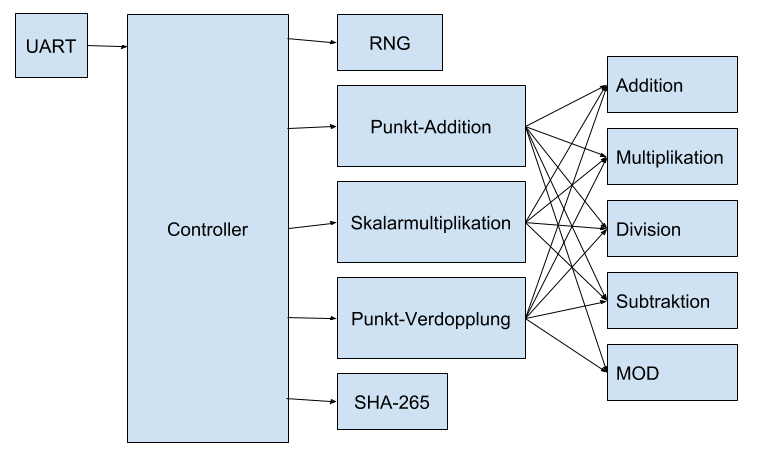
\includegraphics[width=0.9\textwidth]{bilder/opmodules}
	\caption{Zielarchitektur der FPGA-Hardware}
	\label{fig:arch}
\end{figure}

Abbildung \ref{fig:arch} zeigt einen zentralen Controller, der die einzelnen Module benutzt. Der Controller spricht dabei die mathematischen Module an, die konkret für die ECDSA-Implementierung benötigt werden. Dazu werden die atomaren Operationen (Addition, Multiplikation, Division, Subtraktion, Modulo) jeweils eingebunden, um ein höheres Abstraktionsniveau zu erhalten. Das UART-Modul repräsentiert die Kommunikation nach außen. \\

Um den ECDS-Algorithmus optimal zu implementieren, muss auf der Hardware ein ``echter'' Zufallszahlengenerator\footnote{engl. Random Number Generator, RNG} vorhanden sein, um den geheimen Schlüssel richtig zu generieren. Außerdem soll der Controller mit einer beliebig langen Nachricht umgehen und den Algorithmus zum Signieren auf einem kryptographisch sicheren Hashwert ausführen können. Da der Fokus dieser Arbeit auf Implementierung und Vergleich der ECDSA-Kernkomponenten liegt, wird aus Komplexitäts- und Platzgründen\footnote{Chipfläche auf dem zur Verfügung stehenden FPGA} auf beide vorangegangenen Features verzichtet. \\

Die Hardware-Implementierung kann eine Nachricht konstanter Länge, der einem Hash der eigentlichen Nachricht entspricht, entgegennehmen und sendet nach der Berechnung den Punkt $(r,s)$ als Antwort zurück. Bei der Verifizierung werden Nachricht und die Werte $r$ und $s$ entgegen genommen und das Ergebnis der Verifizierung (wahr oder falsch) zurück geschickt. \\

\begin{figure}[thb]
	\centering
  	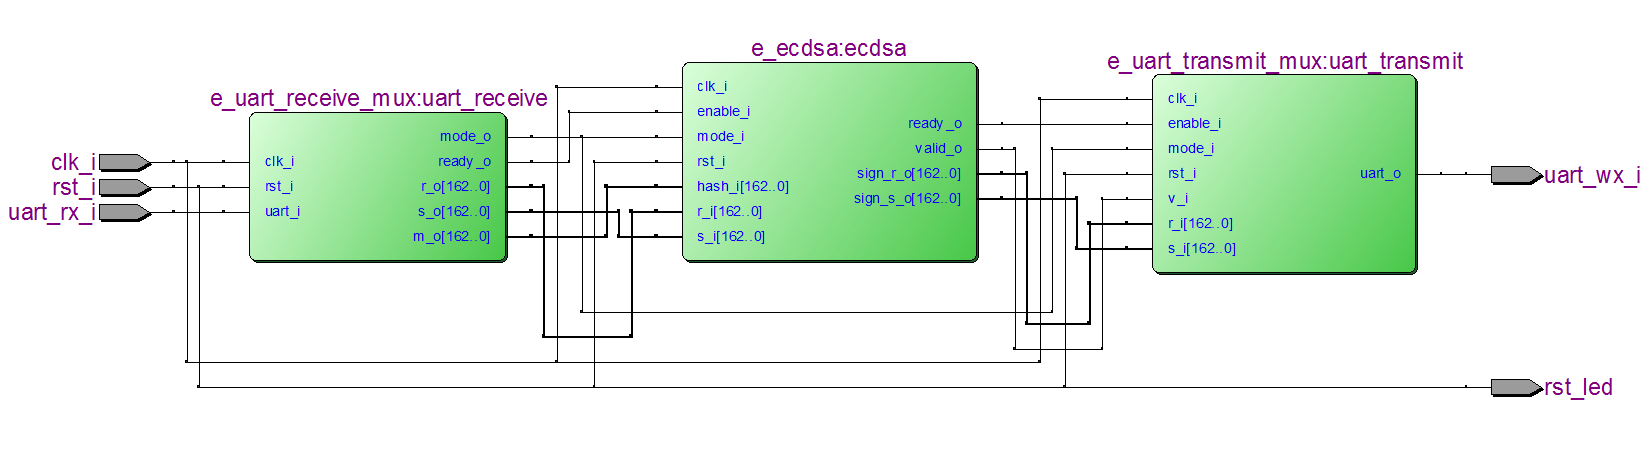
\includegraphics[width=\textwidth]{bilder/tle}
	\caption{Top-Level-Entity der VHDL-Lösung des ECDSA}
	\label{fig:tle}
\end{figure}

Die Top-Level-Entität erhält die Daten über eine serielle RS232-Schnittstelle im Modul \texttt{e\_uart\_receive\_mux} (vgl. Abb. \ref{fig:arch}). Nach vollständigem Erhalt der Daten werden diese dem zentralen Modul \texttt{e\_ecdsa} bereitgestellt und die Berechnung über ein Flag gestartet. Signalisiert das Modul die Fertigstellung der Berechnungen, wird das Modul \texttt{e\_uart\_transmit\_mux} getriggert, welches die Übertragung des Ergebnisses durchführt (vgl. Kap. \ref{sec:uart}). \\


%%%%%%%%%%%%%%%%%%%%%%%%%%%%%%%%%%%%%%%%%%%%%%%%%%%%%%%%%%%%%
\section{VHDL-Komponenten}

% TODO: die wichtigsten komponenten als subsection erklären
\subsection{ECDSA Komponenten...}


\subsection{Kommunikation der UART-Verbindung} \label{sec:uart}



%%%%%%%%%%%%%%%%%%%%%%%%%%%%%%%%%%%%%%%%%%%%%%%%%%%%%%%%%%%%%
\section{Synthetisierung}


%%%%%%%%%%%%%%%%%%%%%%%%%%%%%%%%%%%%%%%%%%%%%%%%%%%%%%%%%%%%%
% bei bedarf hier was zur C-Implementierung schreiben, ansonsten unter Messung -> C
%\section{C-Implementierung} 


